\section{アジャイルソフトウェア開発の実践方法}

アジャイルソフトウェア開発を導入する理由として、4つの前提条件があることを前節で示した。その4つの前提条件を満たすために、アジャイルソフトウェア開発ではウォーターフォールと異なる開発工程と、その工程を実行するための組織と、組織が習慣づけるべき開発技法について言及している。

開発工程はウォーターフォールと異なり、1〜2週間の期間で要求分析、設計、実装、テストを行い、その期間を何度も繰り返すことによってソフトウェアを開発して行く。またこの1~2週間の期間のことをイテレーション (もしくはスプリント)と呼ぶ。

\begin{figure}[H]
\centering
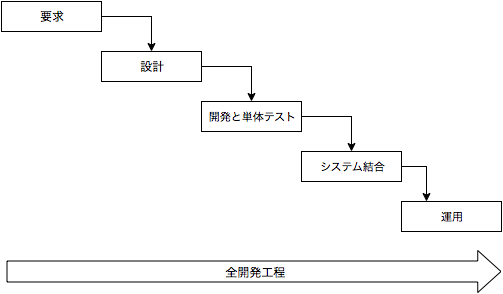
\includegraphics[height=5cm]{./assets/images/waterfall.png}
\caption{ウォーターフォール開発の開発工程}
\label{fig:waterfall}
\end{figure}

\begin{figure}[H]
\centering
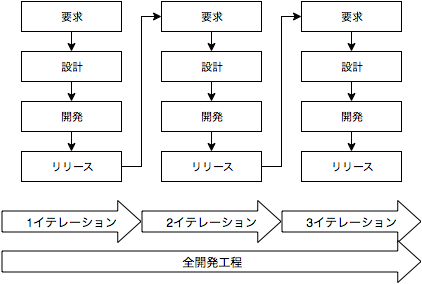
\includegraphics[height=5cm]{./assets/images/agile.png}
\caption{アジャイルソフトウェア開発の開発工程}
\label{fig:agile}
\end{figure}


イテレーションに沿って開発を行うチームは、チームを組織するメンバーで開発に関わる全ての工程をまかなうことが可能である事が望ましいとされている。

文献中 (アジャイルサムライ) 中で、開発チームが定められたイテレーション内で実行すべき (習慣づけるべき) とされている開発技法は以下が挙げられる。

\begin{itemize}
 \item[・]テスト駆動開発の実践
 \item[・]継続的インテグレーション
\end{itemize}

\subsection{テスト駆動開発の実践}

これから作成するプロダクトコード\footnote{}に対して、自動で実行可能なユニットテスト\footnote{}を先に記述し、あるべきユニットテストが失敗する状態を作った後に、プロダクトコードの記述を行いユニットテストが成功するようする。テストが成功したらプログラムをリファクタリング\footnote{}し、コードの質上げる。この一連の流れはテストをサポートするためのツールが失敗する際に赤、テストが成功した時に緑色の出力をすることから、「RED, GREEN, リファクタリング」とも呼ばれる。

このテスト駆動開発を実践することにより得られるメリットは3つある。1つめはプロダクトコードに対して無駄なバグを混入させることを減らすこと、2つめはプロダクトコードを変更した際の影響を素早く確認ができる。3つめでメリットとして最も大きいことは、作成したプログラムが安定していること確認できることによって安心感を得られることである。

\subsection{継続的インテグレーション}


従来の開発方法では、ある程度の開発が終了した段階で、ソフトウェアの結合を行っていた。しかし、結合すべきコードが多く、その結果ソフトウェアの結合の失敗が起き、結合失敗による結合に対するネガティブな気持ちの発生および、それに伴う結合の先送りと結合すべきコードの増大、結合失敗と負のスパイラルを生んでいた。それを対処するための継続的インテグレーションとは

\begin{quote}

  開発者がソフトウェアに加えた変更を取り込んで、ソフトウェア全体として統合する作業を途切れること無く続けていく取り組みのことを、継続的インテグレーションと呼ぶ。

\end{quote}

と文献\cite{西村直人2011アジャイルサムライ}の中で述べられている。つまりソフトウェア開発の1フェーズとして、コードの統合フェーズを設けることなく、日常的にソフトウェアを統合することをさし、そのためには、ソースコードのバージョン管理システム\footnote{}や結合するソフトウェアの粒度を小さくする姿勢、ソフトウェアのビルドの自動化などが求められる。
